\documentclass[9pt,a4paper]{article}

\usepackage[a4paper,margin=17mm]{geometry}
\usepackage{fontspec}
\usepackage{xeCJK}
\usepackage{amsmath}
\usepackage{amssymb}
\usepackage{booktabs}
\usepackage{array}
\usepackage{enumitem}
\usepackage{tikz}
\usetikzlibrary{arrows.meta,positioning}

\setmainfont{Noto Serif CJK KR}
\setsansfont{Noto Sans CJK KR}
\setmonofont{Noto Sans Mono CJK KR}
\setCJKmainfont{Noto Serif CJK KR}
\setCJKsansfont{Noto Sans CJK KR}
\setCJKmonofont{Noto Sans Mono CJK KR}

\setlength{\parindent}{0pt}
\setlength{\parskip}{0.30em}
\setlist[itemize]{leftmargin=1.15em,itemsep=0.05em,topsep=0.05em}

\title{\vspace{-2.0em}Imitation Learning Model}
\author{BI lab IL team}
\date{\vspace{-0.8em}\today}

\begin{document}
\maketitle
\vspace{-2.0em}

\section{Input/Output Structure}

This policy is a visuomotor imitation learning model trained from demonstration
trajectories. The model conditions on a short observation history and generates a
short-horizon action trajectory. In the current configuration,
$n_{\mathrm{obs}}=2$, $H=16$, and $n_{\mathrm{act}}=8$.

\[
o_{t-1:t}
=
\left(
I_{t-1:t}^{front},\,
I_{t-1:t}^{wrist},\,
s_{t-1:t}
\right),
\qquad
\hat{A}_{t:t+H-1} = \pi_\theta(o_{t-1:t})
\]

\begin{table}[h]
\centering
\small
\begin{tabular}{p{0.32\linewidth} p{0.24\linewidth} p{0.34\linewidth}}
\toprule
\textbf{Feature} & \textbf{Temporal Shape} & \textbf{Role} \\
\midrule
Front RGB image history & $2 \times 3 \times 480 \times 640$ & Global visual context \\
Wrist RGB image history & $2 \times 3 \times 480 \times 640$ & Local visual context \\
Robot state history & $2 \times 26$ & Arm 6 DoF + hand 20 DoF state \\
Generated action trajectory & $16 \times 26$ & Horizon-level action prediction \\
Execution action chunk & $8 \times 26$ & Actions queued for execution \\
Per-step command & $26$ & One arm/hand joint target sent at a control step \\
\bottomrule
\end{tabular}
\caption{Temporal input/output structure}
\end{table}

The state and action share the same 26D joint space. The model does not output a
Cartesian waypoint or a symbolic command. It predicts target joint vectors directly,
with arm motion and hand motion represented as one coordinated action space.

\begin{center}
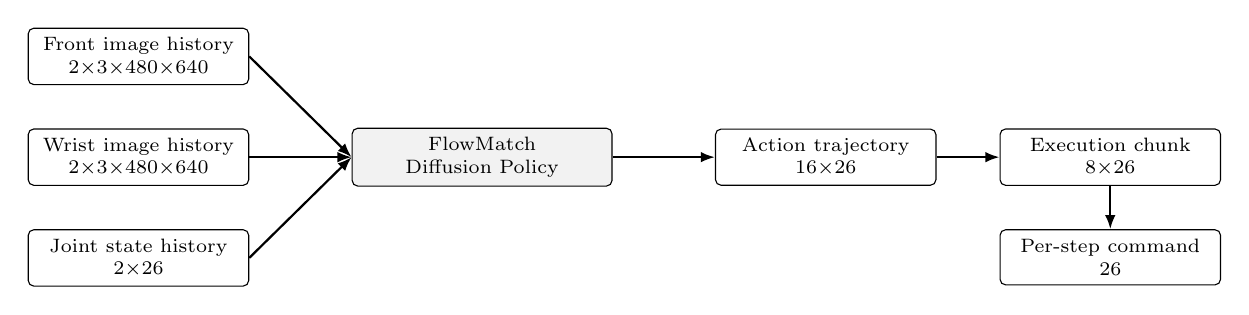
\begin{tikzpicture}[
  node distance=5.5mm and 7.5mm,
  box/.style={draw, rounded corners=2pt, minimum height=7mm, align=center, font=\scriptsize},
  input/.style={box, minimum width=28mm},
  main/.style={box, fill=gray!10, minimum width=33mm},
  arrow/.style={-{Latex[length=1.8mm]}, thick}
]
\node[input] (front) {Front image history\\$2{\times}3{\times}480{\times}640$};
\node[input, below=of front] (wrist) {Wrist image history\\$2{\times}3{\times}480{\times}640$};
\node[input, below=of wrist] (state) {Joint state history\\$2{\times}26$};
\node[main, right=13mm of wrist] (policy) {FlowMatch\\Diffusion Policy};
\node[input, right=13mm of policy] (traj) {Action trajectory\\$16{\times}26$};
\node[input, right=8mm of traj] (chunk) {Execution chunk\\$8{\times}26$};
\node[input, below=of chunk] (cmd) {Per-step command\\$26$};

\draw[arrow] (front.east) -- (policy.west);
\draw[arrow] (wrist.east) -- (policy.west);
\draw[arrow] (state.east) -- (policy.west);
\draw[arrow] (policy.east) -- (traj.west);
\draw[arrow] (traj.east) -- (chunk.west);
\draw[arrow] (chunk.south) -- (cmd.north);
\end{tikzpicture}
\end{center}

\section{Temporal Action Generation}

The generated trajectory has shape $H \times D_a = 16 \times 26$. At inference time,
the policy extracts the execution window starting from the current observation index:

\[
\hat{A}_{t:t+15} \in \mathbb{R}^{16 \times 26},
\qquad
A^{exec}_{t:t+7} \in \mathbb{R}^{8 \times 26},
\qquad
a_t \in \mathbb{R}^{26}.
\]

Thus, the model-level output is a short action trajectory, while the control-level
output at each step is a single 26D joint command. This design preserves short-term
motion intent and temporal consistency across successive arm/hand commands.

\end{document}
